% VISUAL-MANAGED-FILE
% Framing and institutional setting. Sources: Krugman (1980); Flandreau and Jobst (2009); project route-release audit.

% EVIDENCE-STATUS: authentic transaction and route-component trace; exact same-state alternative remains outside this exhibit
% EVIDENCE-COMMIT: ab2c76231653b447c7b151b8d9b4a3fdd7b413e8
% EVIDENCE-SOURCES: output/exhibits/route_replay.json; data/unified/20260110.parquet; https://eth.blockscout.com/tx/0xbda1d07f17c503b5a9c8117c5d1383472006af8a9e22aa4e5e30804b9bf67ad9?tab=token_transfers (retrieved 2026-08-14)
% EVIDENCE-GENERATION: transaction 0xbda1d07f17c503b5a9c8117c5d1383472006af8a9e22aa4e5e30804b9bf67ad9 component 0; partition sha256 a6870bc64badeecf030a1096e69b2ddfc9202e5c4ef99a8c5237d4d458033c6d
% LIVE-COMPANION: output/live/route_replay.html (native HTML/CSS/JS reveal; no embedded video)
% LITERATURE-PRECEDENT: Lehar and Parlour (2025), Appendix B, pairs one named explorer transaction with decoded logs before handing off to the population reconstruction.
% VISUAL-FUNCTION: source-versus-pool-route handoff | authentic explorer screenshot plus settlement trace | separate the user's PYUSD instruction from the USDC-funded pool component
% Generated from output/exhibits/route_replay.json; do not edit by hand.
\newcommand{\RouteReplayInputAmount}{459,930}
\newcommand{\RouteReplayVehicleAmount}{460,331}
\newcommand{\RouteReplayOutputAmount}{460,104}
\newcommand{\RouteReplayValue}{459,930}

\begin{frame}{The PYUSD swap reaches a USDC-funded pool route}
\evidencekicker{User instruction recorded by the explorer}
\vspace{0.02cm}
\centering
\fcolorbox{rule}{white}{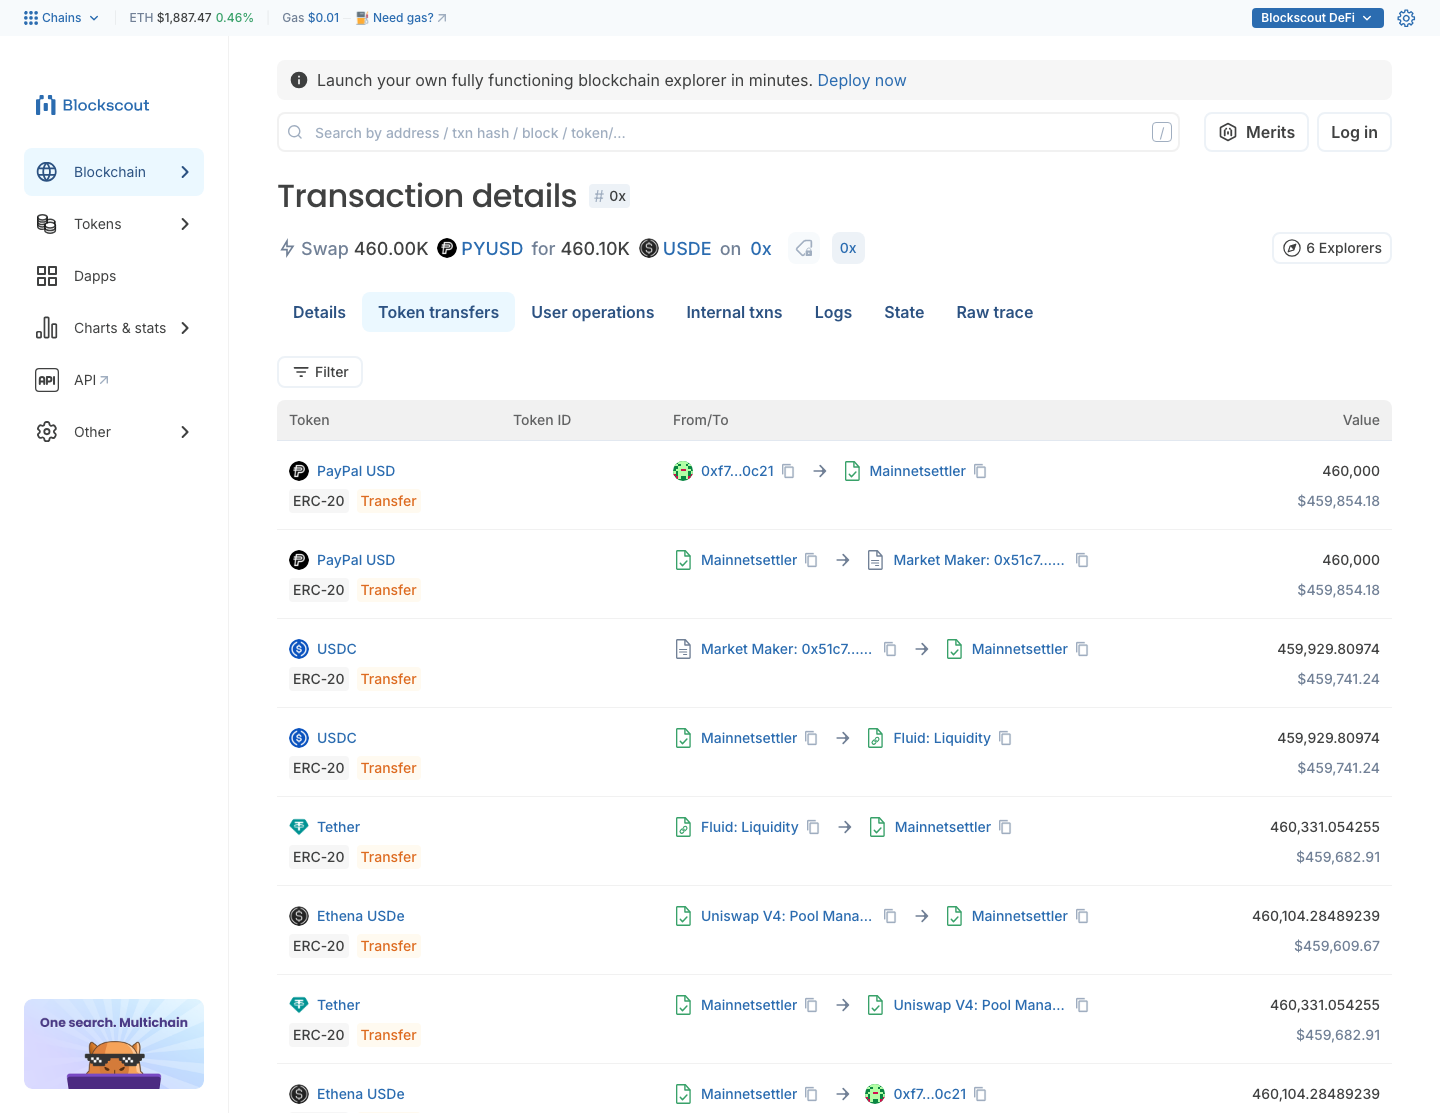
\includegraphics[width=0.88\textwidth,height=1.38cm,keepaspectratio,trim=270 820 430 170,clip]{assets/observed_route_blockscout.png}}
\par\vspace{0.15cm}
\evidencekicker{The decisive settlement transfers}
\vspace{0.02cm}
\fcolorbox{rule}{white}{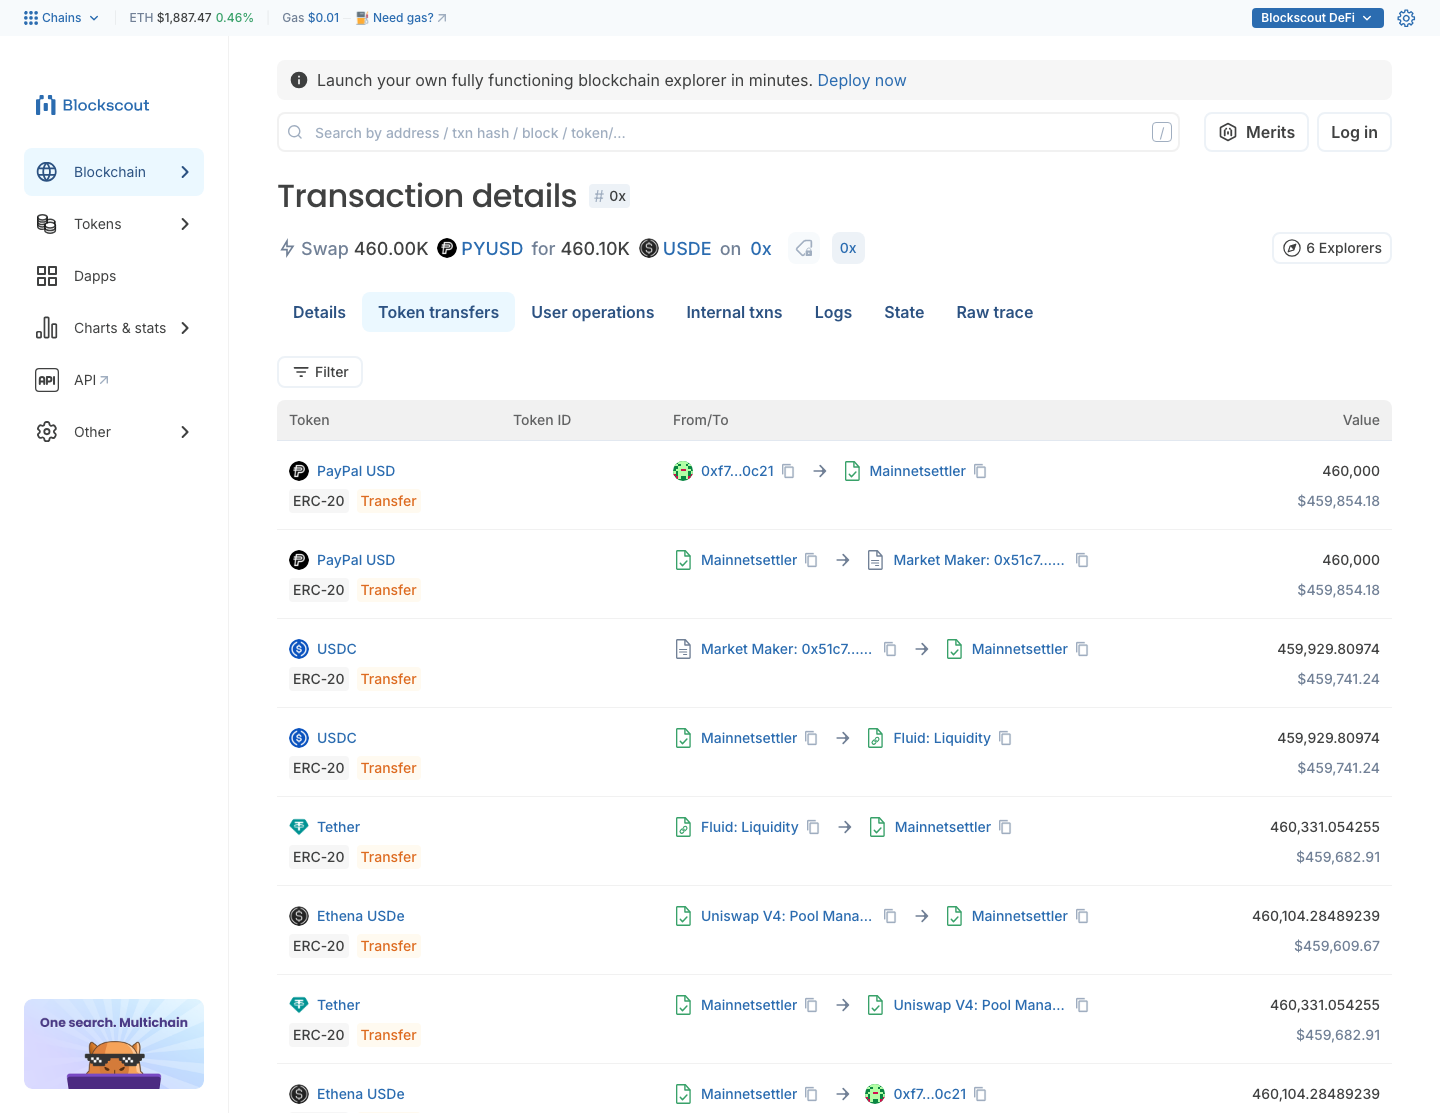
\includegraphics[width=0.94\textwidth,height=1.04cm,keepaspectratio,trim=280 415 324 615,clip]{assets/observed_route_blockscout.png}}
\par\vspace{0.08cm}
\fcolorbox{rule}{white}{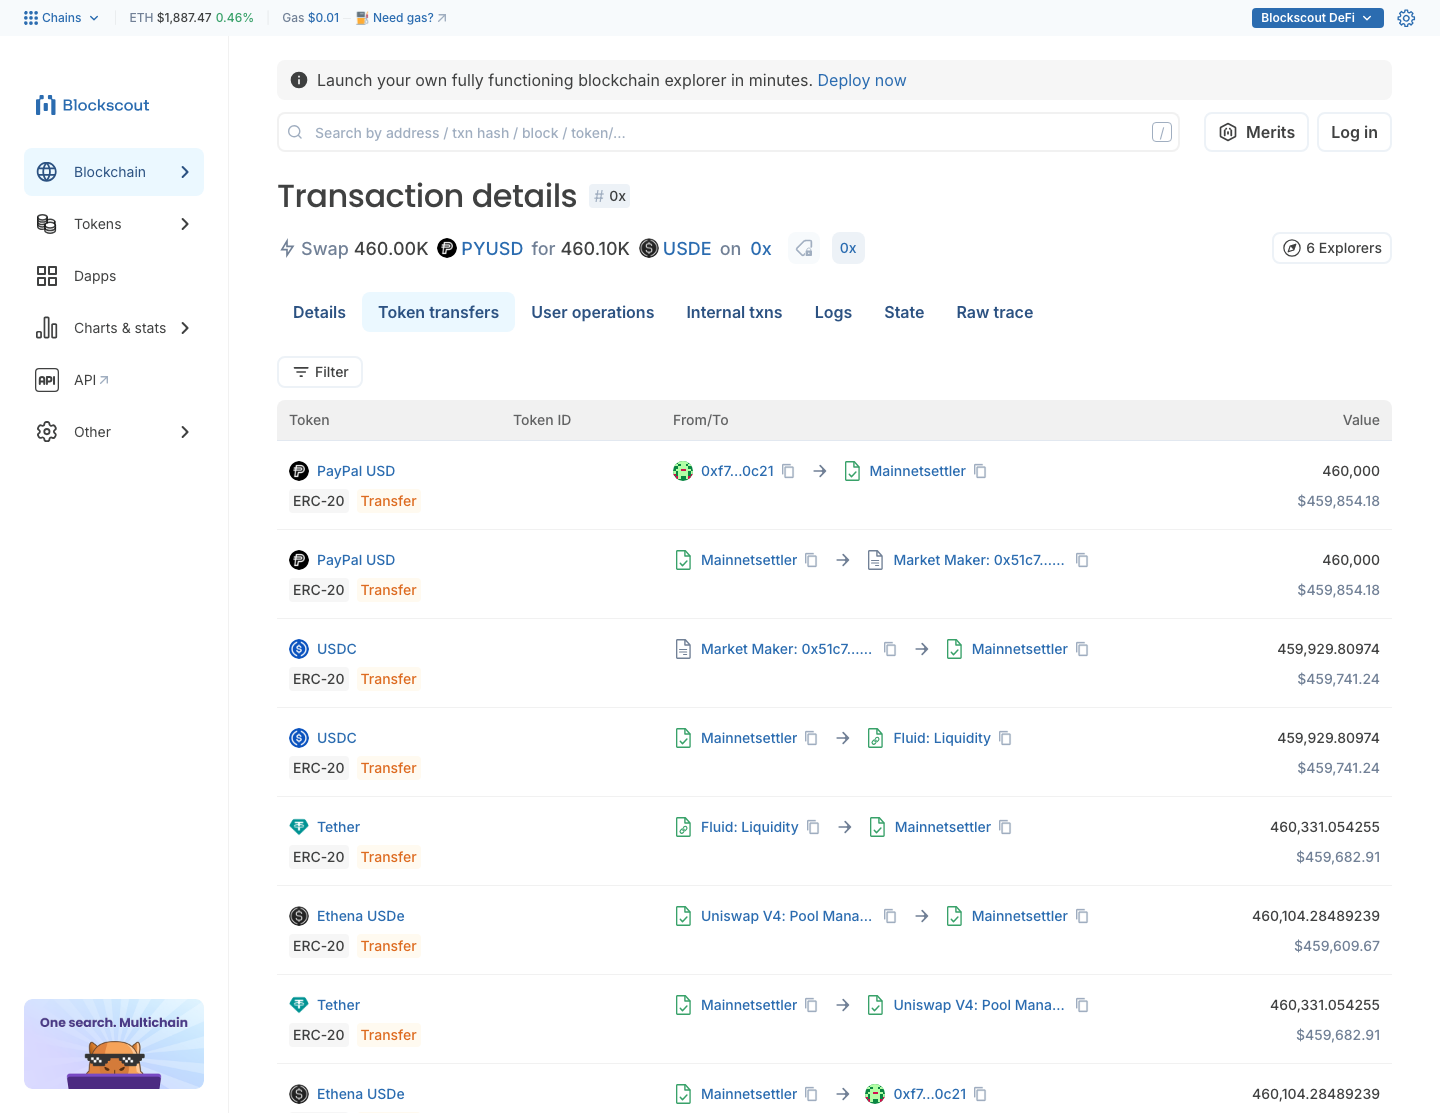
\includegraphics[width=0.94\textwidth,height=1.04cm,keepaspectratio,trim=280 320 324 700,clip]{assets/observed_route_blockscout.png}}
\par\vspace{0.14cm}
{\normalsize\raggedright The instruction is PYUSD $\rightarrow$ USDe. The maker supplies the USDC used by the Fluid leg, which begins the connected pool route.\par}
\decknote{The explorer screenshot and transfer trace refer to transaction \ethtx{0xbda1d07f17c503b5a9c8117c5d1383472006af8a9e22aa4e5e30804b9bf67ad9}{0xbda1d07f\ldots 9bf67ad9} on 10 January 2026.}
\end{frame}

% EVIDENCE-STATUS: authentic connected pool-swap component from the same transaction; exact same-state alternative remains outside this exhibit
% EVIDENCE-COMMIT: ab2c76231653b447c7b151b8d9b4a3fdd7b413e8
% EVIDENCE-SOURCES: output/exhibits/route_replay.json; data/unified/20260110.parquet
% EVIDENCE-GENERATION: transaction 0xbda1d07f17c503b5a9c8117c5d1383472006af8a9e22aa4e5e30804b9bf67ad9 component 0; partition sha256 a6870bc64badeecf030a1096e69b2ddfc9202e5c4ef99a8c5237d4d458033c6d
% VISUAL-FUNCTION: observed vehicle use | source-versus-pool-route breadcrumb plus native connected-route diagram | define the component endpoints and intermediary used in the vehicle-dominance measure
\begin{frame}{Inside the pools, USDT links USDC to USDe}
\centering
\vspace{-0.05cm}
\evidencekicker{Ordered transfers and route reconstruction}
\vspace{0.06cm}
\begin{tikzpicture}[x=1cm,y=1cm]
\node[softbox,inner sep=4pt,text width=3.35cm,minimum height=0.58cm,align=center] (user) at (2.75,0) {\scriptsize User instruction: PYUSD $\rightarrow$ USDe};
\node[font=\small\bfseries,text=muted] at (5.20,0) {$\Longrightarrow$};
\node[softbox,inner sep=4pt,draw=stable,text width=4.15cm,minimum height=0.58cm,align=center] (pools) at (8.30,0) {\scriptsize Pool route: USDC $\rightarrow$ USDT $\rightarrow$ USDe};
\end{tikzpicture}
\vspace{0.20cm}
\begin{tikzpicture}[x=1cm,y=1cm]
\node[nodepoint,minimum size=46pt,font=\small\bfseries] (a) at (1.30,3.25) {USDC};
\node[nodepoint,fill=ucldark,text=white,draw=ucldark,minimum size=46pt,font=\small\bfseries] (k) at (6.15,3.25) {USDT};
\node[nodepoint,minimum size=46pt,font=\small\bfseries] (b) at (11.00,3.25) {USDe};
\draw[route,draw=ucldark,line width=1.8pt] (a)--(k);
\draw[route,draw=ucldark,line width=1.8pt] (k)--(b);
\node[font=\normalsize\bfseries,text=ucldark,align=center] at (3.72,4.18) {Fluid};
\node[font=\normalsize\bfseries,text=ucldark,align=center] at (8.57,4.18) {Uniswap V4};
\node[font=\small,text=muted,align=center] at (3.72,2.31) {\RouteReplayInputAmount{} USDC\\$\rightarrow$ \RouteReplayVehicleAmount{} USDT};
\node[font=\small,text=muted,align=center] at (8.57,2.31) {\RouteReplayVehicleAmount{} USDT\\$\rightarrow$ \RouteReplayOutputAmount{} USDe};
\node[font=\scriptsize\bfseries,text=white,fill=ucldark,rounded corners=2pt,inner sep=4pt] at (6.15,1.15) {vehicle};
\end{tikzpicture}
\vspace{0.15cm}
\begin{minipage}{0.78\textwidth}
\centering
{\small Our route sample begins with USDC, the source asset of the connected pool-swap component. USDT is the vehicle because it links the two legs.\par}
\end{minipage}
\par\vspace{0.04cm}
{\raggedright\decknote{The route is the connected pool-swap component of transaction \ethtx{0xbda1d07f17c503b5a9c8117c5d1383472006af8a9e22aa4e5e30804b9bf67ad9}{0xbda1d07f\ldots 9bf67ad9} on 10 January 2026.}}
\end{frame}

% VISUAL-FUNCTION: dominance denominator | route glyph plus paired measure definitions | separate count, value, and network position
\begin{frame}{Vehicle dominance is the share of indirect trade carried by an asset}
\begin{columns}[T,totalwidth=\textwidth]
\begin{column}{0.43\textwidth}
\evidencekicker{Measurement}
\begin{itemize}
\item Dominance is the share of indirect trade intermediated by asset $k$.
\item Count share treats each route equally; value share weights routes by dollar value.
\item Network measures capture how broadly $k$ connects endpoint pairs.
\end{itemize}
\end{column}
\begin{column}{0.53\textwidth}
\centering
\begin{tikzpicture}[x=1cm,y=1cm]
\node[nodepoint] (a) at (0,3.45) {$i$};
\node[nodepoint,fill=ucldark,text=white,draw=ucldark] (k) at (2.0,3.45) {$k$};
\node[nodepoint] (b) at (4.0,3.45) {$o$};
\draw[route] (a) -- (k);
\draw[route] (k) -- (b);
\node[anchor=west,font=\small\bfseries,text=ucldark] at (0,2.10) {Count-weighted dominance};
\node[anchor=west,font=\small,align=left,text width=6.0cm] at (0,1.58) {Share of indirect routes that pass through $k$};
\node[anchor=west,font=\small\bfseries,text=stable] at (0,0.78) {Value-weighted dominance};
\node[anchor=west,font=\small,align=left,text width=6.0cm] at (0,0.26) {Share of comparable routed value that passes through $k$};
\end{tikzpicture}
\end{column}
\end{columns}
\end{frame}

% EVIDENCE-STATUS: verified institutional mechanism; no empirical estimate is displayed.
% SOURCE-GENERATION: repository HEAD eac25258ea36.
% SOURCE: docs/finding-v1-forced-vehicle.md sha256=650004eafae8864fe13b3d90ab59daefd77b342e33510f3d5db03b3e28ed2c68 (V1/V2 pairing contract).
% SOURCE: literature/text/2021-AdamsZinsmeisterRobinson2021UniswapV3-whitepaper-uniswap-v3-core.txt sha256=599a20254f8d5f1d6e771d2899bf16e4a921c5bc3a9cb82e58c97d7791411567 (V3 ranges, ticks, and fee tiers).
% SOURCE: https://app.uniswap.org/whitepaper-v4.pdf, Adams et al. (2024), Uniswap v4 Core, Sections 1 and 3 (singleton, hooks, and flash accounting).
% SOURCE: docs/research-questions-and-empirical-design.md sha256=b56cb5e98d93d0968306fc2dd36edb323d83519daab17b5c7b39587d49506c8b (V4 settlement boundary).
% SOURCE: src/ddvc/execution_contracts.py sha256=67b28ca58519cf9cef80314211f168989b60502c5a3fb8792ad8814613ddae00 (supported V4 vanilla concentrated-liquidity contract).
% SCIENTIFIC-BOUNDARY: architecture changes feasible pair formation, liquidity placement, or settlement. Pool adoption and realised route use are endogenous exposure, and calendar date alone is not treatment.
% VISUAL-FUNCTION: V1-to-V4 architecture morph | four-panel mechanism strip | separate design, realised exposure, and calendar time
\begin{frame}{Architecture changes routing opportunities}
\setlength{\fboxsep}{5pt}
\setlength{\fboxrule}{0.45pt}
\begin{columns}[T,totalwidth=\textwidth]

% V1: the pairing contract makes ETH the only token-to-token path.
\begin{column}{0.238\textwidth}
\fcolorbox{rule}{panel}{\begin{minipage}[t][3.95cm][t]{0.88\linewidth}
{\small\bfseries\color{ucldark}V1}\hfill{\scriptsize\color{muted}mandatory hub}\par
\vspace{0.18cm}
\centering
\begin{tikzpicture}[tinyasset/.style={circle,draw=ink,fill=white,minimum size=14pt,inner sep=0pt,font=\tiny},routearrow/.style={-{Stealth[length=4pt]},line width=1.15pt}]
\node[tinyasset] (a) at (0,0) {A};
\node[tinyasset,fill=ucldark,text=white,draw=ucldark,minimum size=23pt] (k) at (1.05,0) {ETH};
\node[tinyasset] (b) at (2.10,0) {B};
\draw[routearrow,draw=accent] (a)--(k);
\draw[routearrow,draw=accent] (k)--(b);
\draw[rule,densely dashed] (a) to[bend left=35] node[above,font=\tiny,text=muted] {no direct pool} (b);
\end{tikzpicture}
\par\vspace{0.22cm}
\raggedright\scriptsize Only ETH--token pools: token-to-token execution must pass through ETH.\par
\vfill
{\scriptsize\bfseries\color{accent}Hub use is imposed}\par
\end{minipage}}
\end{column}

% V2: arbitrary pairs add a direct opportunity while leaving vehicle routes feasible.
\begin{column}{0.238\textwidth}
\fcolorbox{rule}{panel}{\begin{minipage}[t][3.95cm][t]{0.88\linewidth}
{\small\bfseries\color{ucldark}V2}\hfill{\scriptsize\color{muted}pair choice}\par
\vspace{0.18cm}
\centering
\begin{tikzpicture}[tinyasset/.style={circle,draw=ink,fill=white,minimum size=14pt,inner sep=0pt,font=\tiny},routearrow/.style={-{Stealth[length=4pt]},line width=1.15pt}]
\node[tinyasset] (a) at (0,0) {A};
\node[tinyasset,fill=ucldark,text=white,draw=ucldark,minimum size=23pt] (k) at (1.05,0) {$k$};
\node[tinyasset] (b) at (2.10,0) {B};
\draw[routearrow,draw=ucldark] (a)--(k);
\draw[routearrow,draw=ucldark] (k)--(b);
\draw[routearrow,draw=stable] (a) to[bend left=35] node[above,font=\tiny,text=stable] {direct} (b);
\end{tikzpicture}
\par\vspace{0.22cm}
\raggedright\scriptsize Arbitrary pairs add a direct route; vehicle routes remain feasible.\par
\vfill
{\scriptsize\bfseries\color{stable}Hub use becomes a choice}\par
\end{minipage}}
\end{column}

% V3: bounded ranges make active depth depend on where liquidity is placed.
\begin{column}{0.238\textwidth}
\fcolorbox{rule}{panel}{\begin{minipage}[t][3.95cm][t]{0.88\linewidth}
{\small\bfseries\color{ucldark}V3}\hfill{\scriptsize\color{muted}range choice}\par
\vspace{0.25cm}
\centering
\begin{tikzpicture}[x=1cm,y=1cm]
\node[anchor=east,font=\tiny] at (0.28,0.27) {A/B};
\draw[rule,line width=0.85pt] (0.38,0.27)--(2.18,0.27);
\draw[stable,line width=3pt] (0.83,0.27)--(1.35,0.27);
\node[anchor=east,font=\tiny] at (0.28,-0.20) {via $k$};
\draw[rule,line width=0.85pt] (0.38,-0.20)--(2.18,-0.20);
\draw[ucldark,line width=3pt] (0.58,-0.20)--(1.08,-0.20);
\draw[uclbright,line width=3pt] (1.48,-0.20)--(2.02,-0.20);
\end{tikzpicture}
\par\vspace{0.28cm}
\raggedright\scriptsize LPs choose ranges and fees; active depth can favor direct pairs or vehicle spokes.\par
\vfill
{\scriptsize\bfseries\color{uclbright}Opportunity shifts by pair}\par
\end{minipage}}
\end{column}

% V4: settlement can net movement without erasing the economic route or its pools.
\begin{column}{0.238\textwidth}
\fcolorbox{rule}{panel}{\begin{minipage}[t][3.95cm][t]{0.88\linewidth}
{\small\bfseries\color{ucldark}V4}\hfill{\scriptsize\color{muted}net settlement}\par
\vspace{0.18cm}
\centering
\begin{tikzpicture}[tinyasset/.style={circle,draw=ink,fill=white,minimum size=14pt,inner sep=0pt,font=\tiny},routearrow/.style={-{Stealth[length=4pt]},line width=1.15pt}]
\node[rounded corners=2pt,draw=uclbright,densely dashed,minimum width=2.45cm,minimum height=0.92cm] at (1.05,0) {};
\node[tinyasset] (a) at (0,0) {A};
\node[tinyasset,fill=ucldark,text=white,draw=ucldark,minimum size=21pt] (k) at (1.05,0) {$k$};
\node[tinyasset] (b) at (2.10,0) {B};
\draw[routearrow,draw=ucldark] (a)--(k);
\draw[routearrow,draw=ucldark] (k)--(b);
\node[anchor=north,font=\tiny,text=uclbright] at (1.05,-0.50) {shared accounting};
\end{tikzpicture}
\par\vspace{0.22cm}
\raggedright\scriptsize Two pools still execute; intermediate token movement may be netted.\par
\vfill
{\scriptsize\bfseries\color{ucldark}Settlement can diverge from route use}\par
\end{minipage}}
\end{column}
\end{columns}

% The empirical design must not substitute the version date for exposure to its mechanism.
\vspace{0.25cm}
\colorbox{panel}{\parbox[c][0.72cm][c]{0.965\textwidth}{\hspace{0.15cm}\scriptsize
\textbf{Architecture}\; feasible rules\hfill
\textbf{Exposure}\; realised pool and route use\hfill
\textbf{Calendar date}\; timing only\hspace{0.15cm}}}
\end{frame}
